\documentclass[pdftex,12pt,a4paper]{article}
\usepackage{multicol}
\usepackage[utf8]{inputenc}
\usepackage[portuguese]{babel}
\usepackage[T1]{fontenc}
\usepackage[numbers]{natbib}
\usepackage{amsmath}
\usepackage{amsfonts}
\usepackage{amssymb}
\usepackage{mathabx}
\usepackage{mathtools}
\usepackage{fancyhdr}
\usepackage{color}
\usepackage[pdftex]{graphicx}
\usepackage{geometry}
\geometry{verbose,tmargin=2.5cm,bmargin=2.5cm,lmargin=2cm,rmargin=2cm}
\usepackage{caption}
\usepackage{subcaption}
\usepackage{sidecap}
\usepackage[labelfont={bf,footnotesize}]{caption}
\usepackage{pdfpages}
\usepackage{hyperref}
\usepackage{bookmark}
\textheight = 700pt
\pagestyle{fancy}
\fancyhf{}
\fancyhead[RO]{\null}
\fancyhead[LE]{\null}
\fancyfoot[RO,LE]{\thepage}
\renewcommand{\headrulewidth}{0pt}
\renewcommand{\footrulewidth}{0pt}
\newcommand{\HRule}{\rule{\linewidth}{0.3mm}}
\textheight = 680pt
\addto\captionsportuguese{\renewcommand{\figurename}{Gráfico}}
\renewcommand{\thefigure}{\arabic{figure}}
\renewcommand{\thetable}{\arabic{table}}
\renewcommand{\theequation}{\arabic{equation}}

\begin{document}
\begin{titlepage}
\begin{center}

~\\[5.0cm]
\textsc{\large Quarta Avaliação}\\
\HRule \\[0.4cm]
{ \huge \bfseries Mapa Logístico e Caos \\[0.4cm] }
\HRule \\[0.5cm]
\textsc{\Large Física Computacional}\\
~\\[3.5cm]
\noindent
\small Aluno\\
\large \textsc Marcos Paulo Gomes De Castro\\[0.2cm]
\small Professor\\
\large \textsc Nuno Crokidakis\\[0.2 cm]
\vfill


\includegraphics[width=1.0cm]{logo}\\

\textsc Universidade Federal Fluminense\\ 
{\normalsize \today}

\end{center}
\end{titlepage}

\section*{Introdução}
 ~~~~~ Um Mapa Logistico é uma aplicação matemática que associa um valor $x_{n+1}$ com outro $x_{n}$, tal objeto foi citado inicialmente em um artigo sobre comportamento caótico em equações não lineares, tendo sua popularização em 1976 em um artigo de  Robert May sobre comportamento demográfico.\
~Oriundo da equações de Pierre François Verhulst:
\begin{equation}
\mathrm{\frac{d}{dt}}x(t) = \lambda x(t)\left(1 - \frac{x(t)}{K}\right),\label{eq:diferencial}
\end{equation}
aqui trataremos $K = 1$, tal que, obtemos o seguinte polinômio de segundo grau:
\begin{equation}
x_{n+1} = \lambda x_n(1-x_n),\label{eq:map}
\end{equation}

~~ Este modelo aparentemente simples é muito rico, nele podemos obter informações importantes  no estudo do comportamento caótico. Os pontos em que o mapa se aproxima do seu valor previsto são ditos atratorese, os quais podemos calcular para um dado domínio, haja visto o comportamento caótico do mapa $(1)$ temos valores de $x^*$ para os quais os pontos são diversos e outros métodos algébricos são utilizados:

\begin{align}
0\leq \lambda \leq 1&\ ,\ x^* = 0\label{eq:0-1}\\
1< \lambda \leq 3&\ ,\ x^* = \frac{\lambda-1}{\lambda}\label{eq:1-3}\\
3< \lambda \leq 4&\ ,\ x^* = x_i,\ \text{com}\ i=1,2,...\label{eq:3-4}\\
\lambda>4&\ ,\ x^*=\text{indefinido}\label{eq:4-inf}
\end{align}

~~ Nos itens seguintes faremos uma anlálise deste mapa para diferentes valores de $\lambda$.
\section{Análise de Convergência}
~~~~~~~ Dado o mapa $(2)$ podemos iterar o mesmo fazendo uso de um recurso coputacional, como um programa em C no caso deste trabalho, para isso iremos obter uma coluna com valores de $x_{n}$ e outra para passos de tempo, onde cada iteração representa $1\ segundo $. Ao plotar estes valores em um plano cartesiano, depositando o tempo sobre a abscissa e os valores de $x_{n}$ sobre a ordenada obtemos uma curva onde podemos observar a convergência para o valor calculado vide a relação $(4)$.\

~~ No gráfico $(1)$ temos $\lambda = 1.01$, para este teremos um valor esperado de $x* = 0.00990$, nele podemos ver que o mapa atige a convergência em torno de $25\ min$. 
\pagebreak
\newpage

\begin{figure}
\centering
\caption{Convergência do Mapa Logístico para $\lambda = 1.01$.}
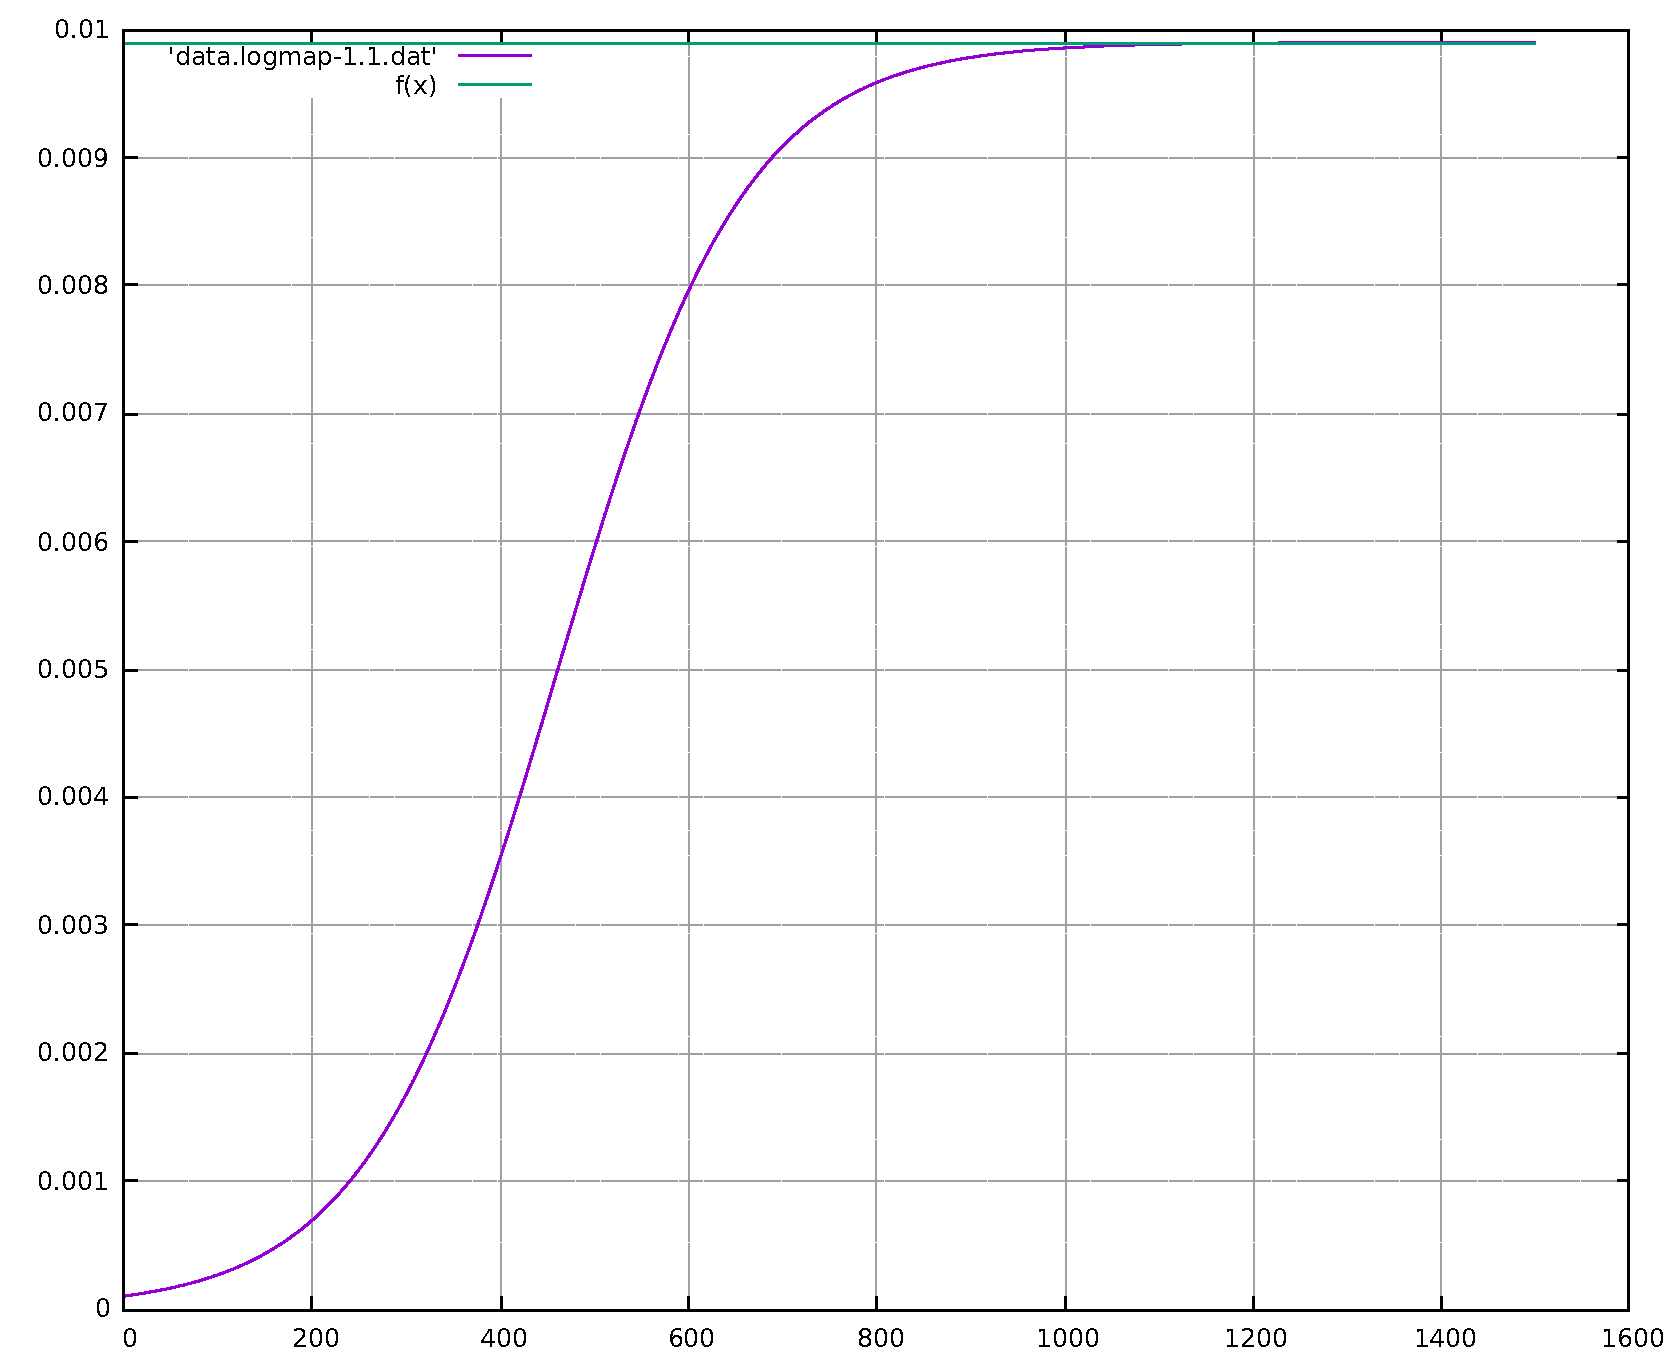
\includegraphics[scale=0.5]{01}
\caption*{$x\ na\ ordenada\ e\ tempo(segundos)\ na\ abscissa$}
\end{figure}

\section{Diagramas e Atratores}
~~~~~~~ Para valores de $ \lambda \geq 1.00$ temos valores de $ x_{n} \geq 0$, com isso podemos plotar um diagrama de $x_{n+1}\ por\ x_{n}$ sobre a reta $x_{n+1} = x_{n}$ e a parábola $x_{n+1} = \lambda x_n(1-x_n)$ e obter diagramas escada para analisar os pontos atratores. Para valores de $1 \leq \lambda \leq 3$ temos pontos simples, onde o mapa logístico converge e atinge os valores esperados pela relação $(4)$.
\pagebreak
\newpage

\begin{figure}
\subsection{Atrator em $\lambda = 0.90, x* = 0$}
\centering
\caption{Mapa Escada $\lambda = 0.90$.}
\resizebox{\columnwidth}{!}{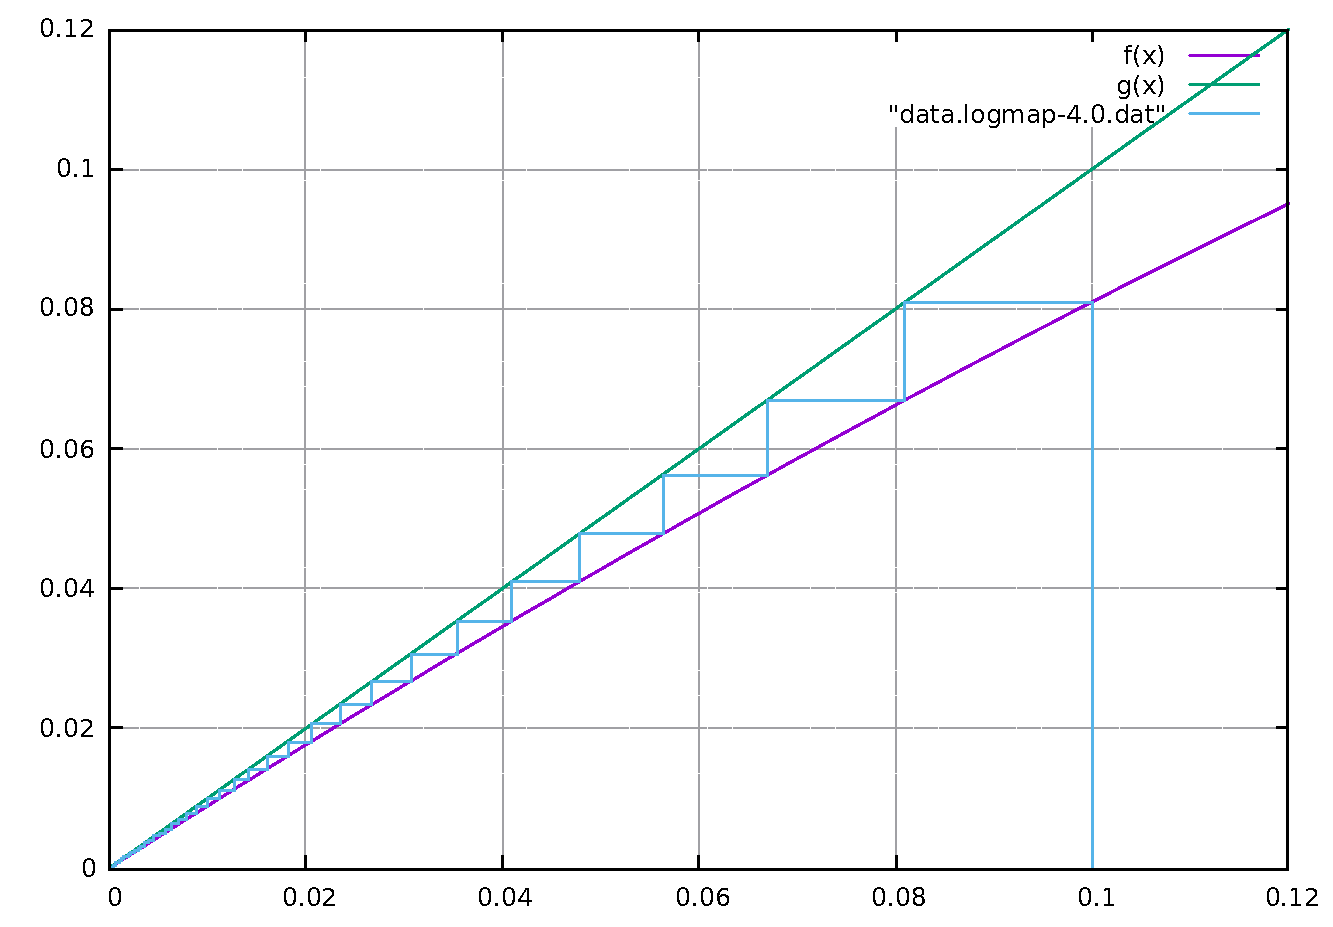
\includegraphics{02}}
\caption*{$x_{n+1}\ na\ ordenada\ e\ x_{n}\ na\ abscissa$ }
\end{figure}
\pagebreak
\newpage

\begin{figure}
\subsection{Atrator em $\lambda = 1.50, x* = 0.33$}
\centering
\caption{Mapa Escada $\lambda = 1.50$.}
\resizebox{\columnwidth}{!}{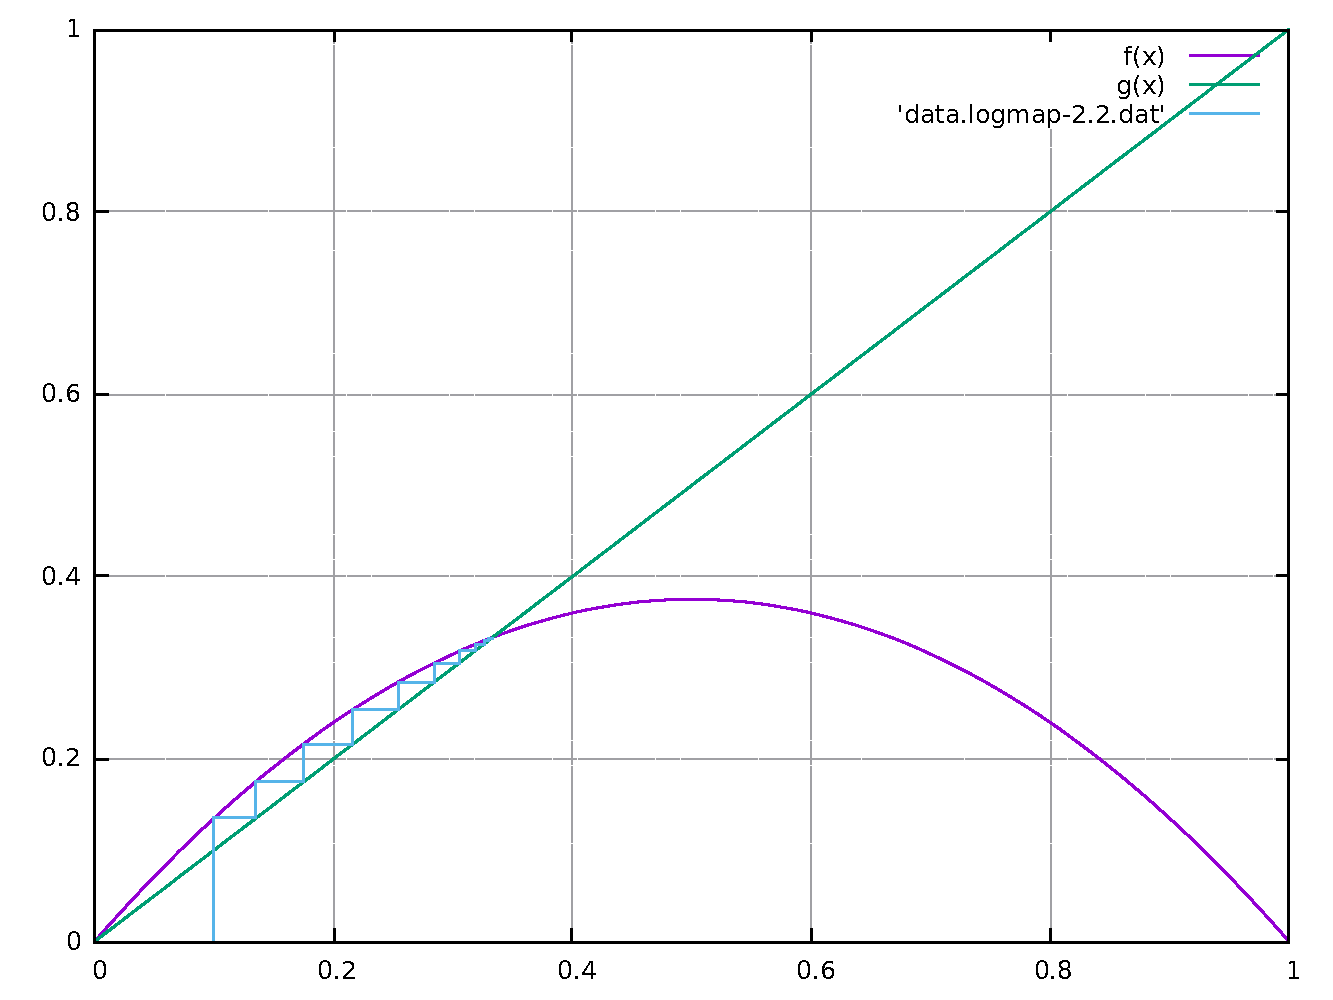
\includegraphics{03}}
\caption*{$x_{n+1}\ na\ ordenada\ e\ x_{n}\ na\ abscissa$ }
\end{figure}
\pagebreak
\newpage

\begin{figure}
\subsection{Atrator em $\lambda = 2.00, x* = 0.50$}
\centering
\caption{Mapa Escada $\lambda = 2.00$.}
\resizebox{\columnwidth}{!}{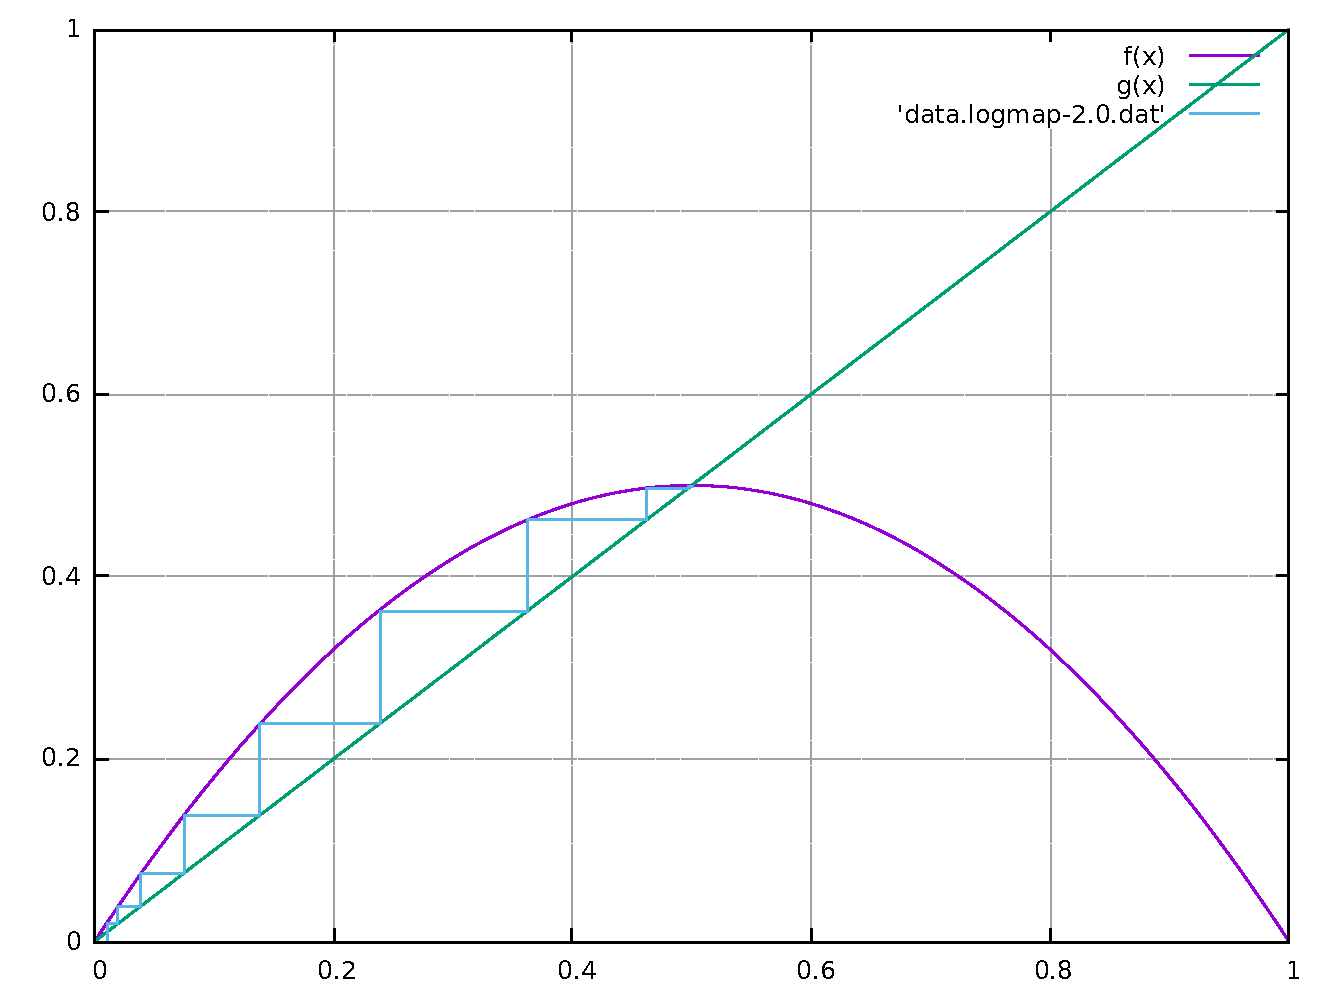
\includegraphics{04}}
\caption*{$x_{n+1}\ na\ ordenada\ e\ x_{n}\ na\ abscissa$ }
\end{figure}

\begin{figure}

\section{Valores Excentricos de $\lambda$}
~~~~~~ Para valores de $3 \leq \lambda \leq 4$ temos um comportamento caótico, surgem outros pontos atratores, e temos de fazer uso de recursos algébricos específicos para determinar analiticamente os seus respectivos valores.\

~~~~~~ O mapa parece convergir para diferentes pontos ao mesmo tempo, em observar a massa de dados obtido pela iteração de $(2)$ podemos ver que os pontos se tornam periódicos, logo no lugar de uma convergência clara o mapa se estabiliza em um equilibrio dinâmico, tendo como pontos atratores os valores tangentes as retas normais.

\subsection{Diagrama para $\lambda = 3.10$}
~~~~~~ Aqui podemos ver o diagrama escada para um dado valor de $\lambda$, onde seus pontos formam uma figura regular seccionando pontos diversos na reta $x'=x$. Este plote não é suficiente para definir os pontos onde o mapa adquire equilibrio dinâmico.\

\centering
\caption{Mapa Escada $\lambda = 3.10$.}
\resizebox{\columnwidth}{!}{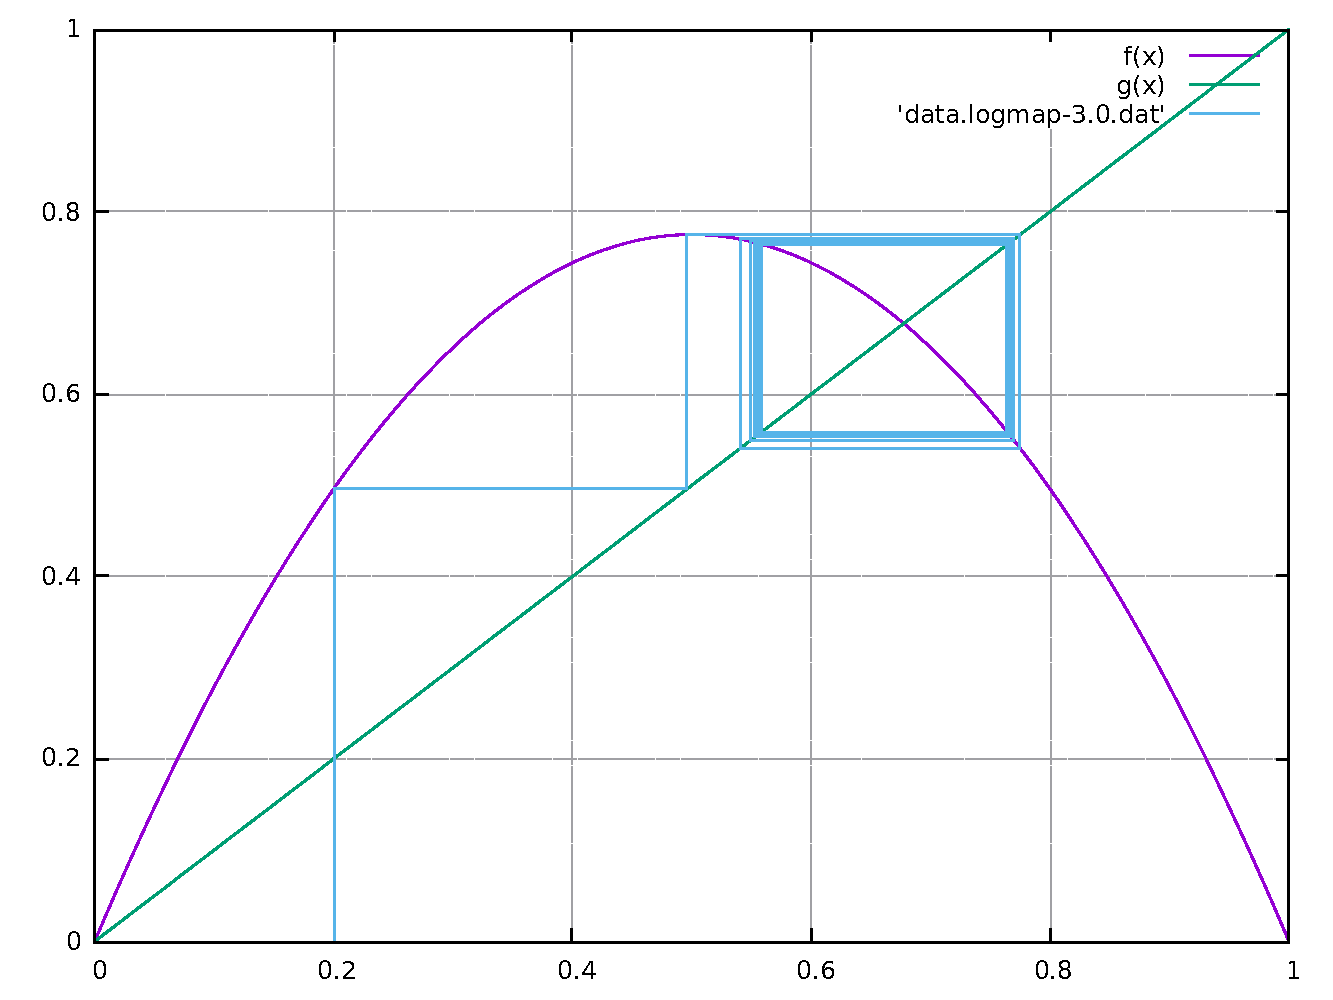
\includegraphics{05}}
\caption*{$x_{n+1}\ na\ ordenada\ e\ x_{n}\ na\ abscissa$ }\ 
\end{figure}

\begin{figure}
~~~~~~ Ao plotar os pontos de $x*$ em função de um tempo, dado que cada passo equivale a $1\ segundo$, obtemos a seguinte relação:

\centering
\caption{Convergência do Mapa Logístico para $\lambda = 3.10$.}
\resizebox{\columnwidth}{!}{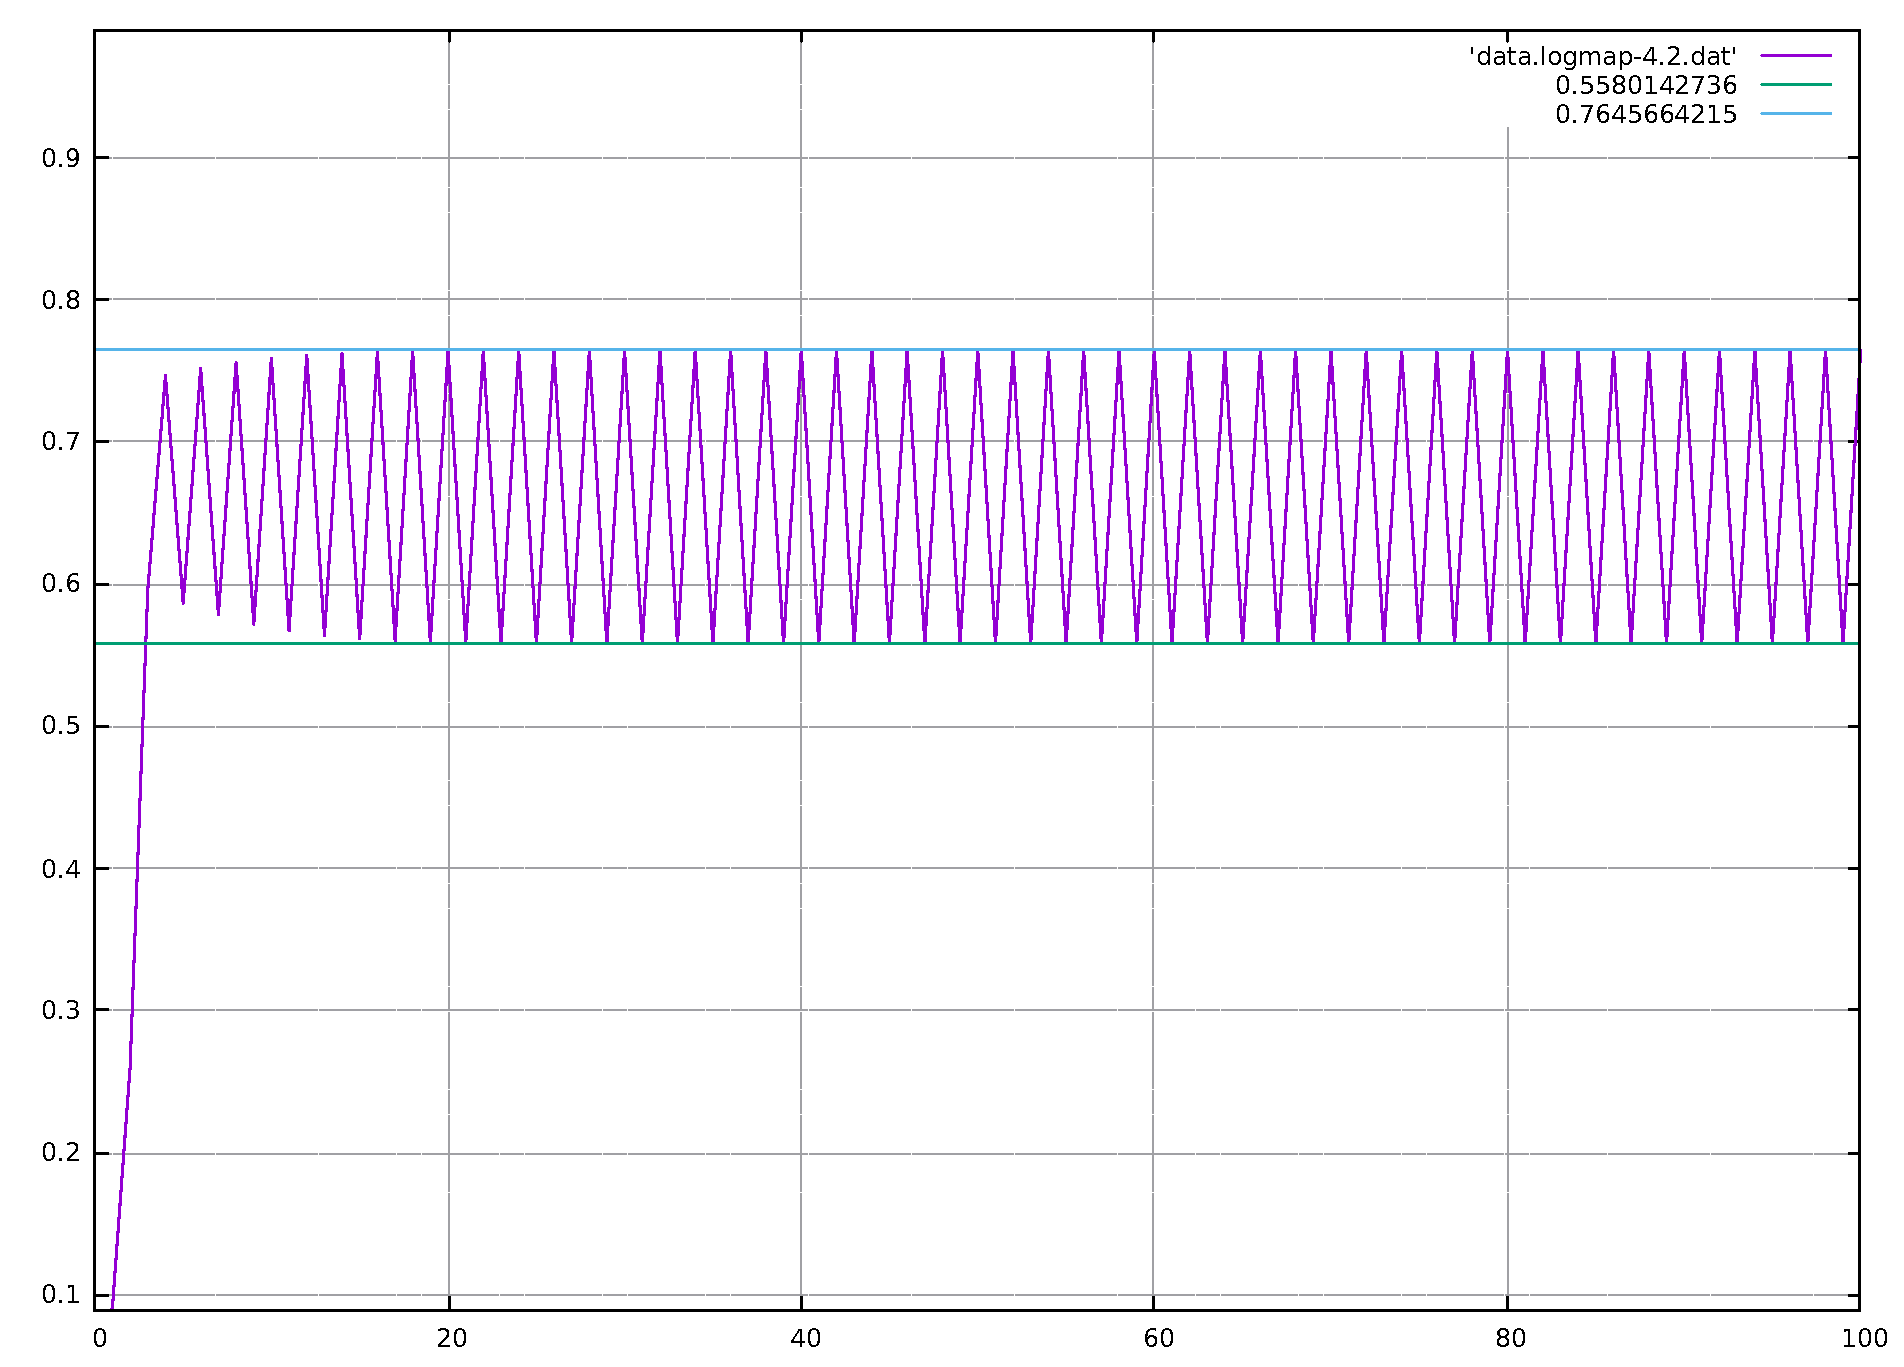
\includegraphics{08}}
\caption*{$x*\ na\ ordenada\ e\ x_{n}\ na\ abscissa$ }\ 

~~~~~~ Aqui vemos apenas dois pontos, mas já podemos observar como o mapa oscila.
\end{figure}

\begin{figure}
\subsection{Diagrama para $\lambda = 3.47$}

~~~~~~ Neste caso temos mais pontos atratores, já é possível ver o quanto os pontos almentam para uma pequena variação em $\lambda$.

\centering
\caption{Mapa Escada $\lambda = 3.47$.}
\resizebox{\columnwidth}{!}{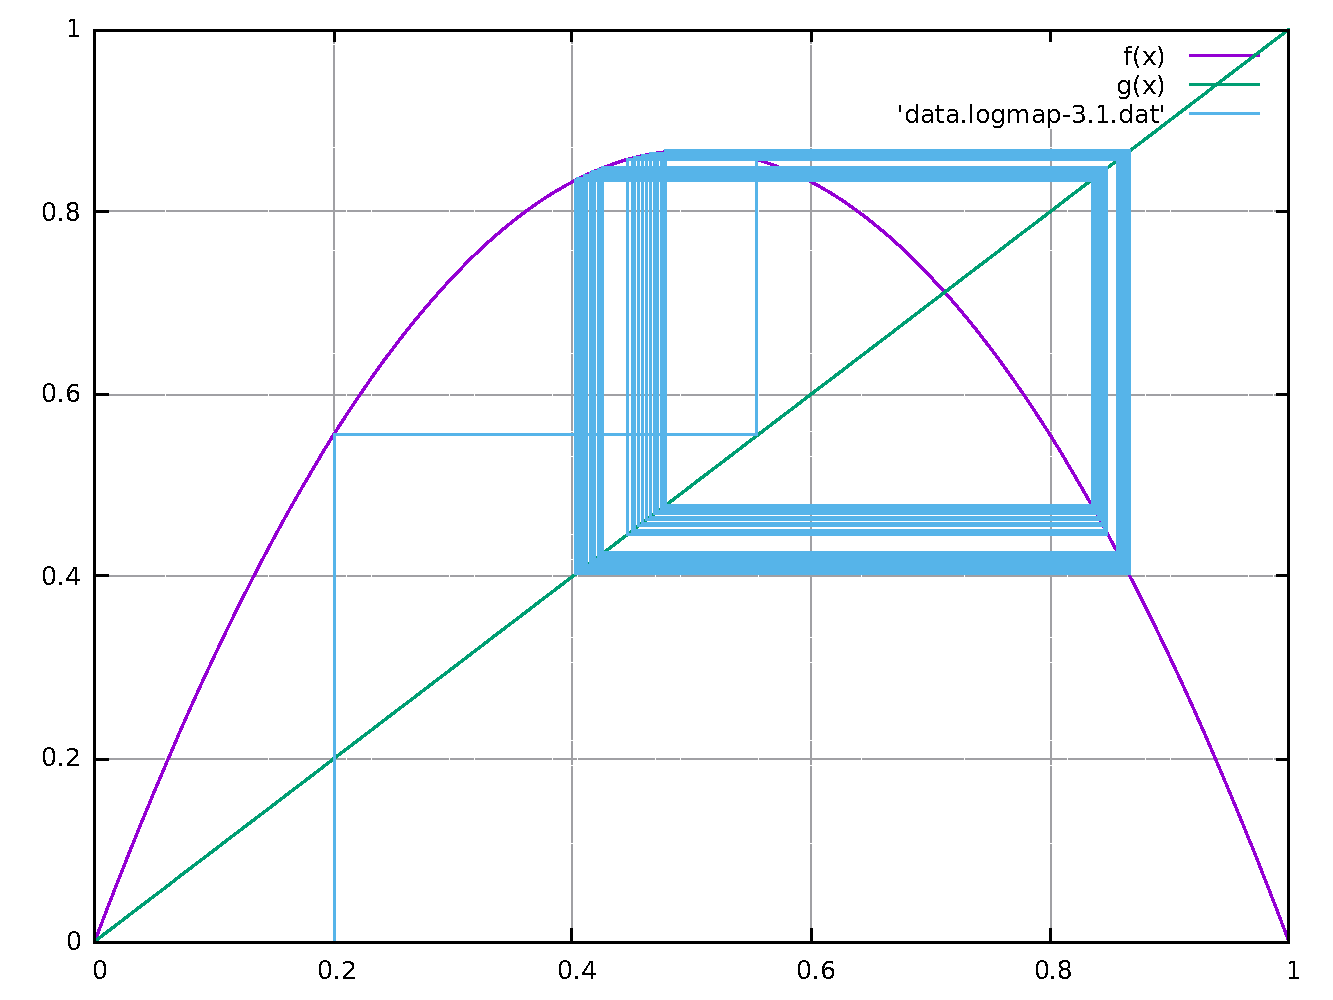
\includegraphics{06}}
\caption*{$x_{n+1}\ na\ ordenada\ e\ x_{n}\ na\ abscissa$ }
\end{figure}

~~~~~~ A oscilação se torna mais excentrica, surgindo maior número de pontos atratores.
\begin{figure}
\centering
\caption{Convergência do Mapa Logístico para $\lambda = 3.47$.}
\resizebox{\columnwidth}{!}{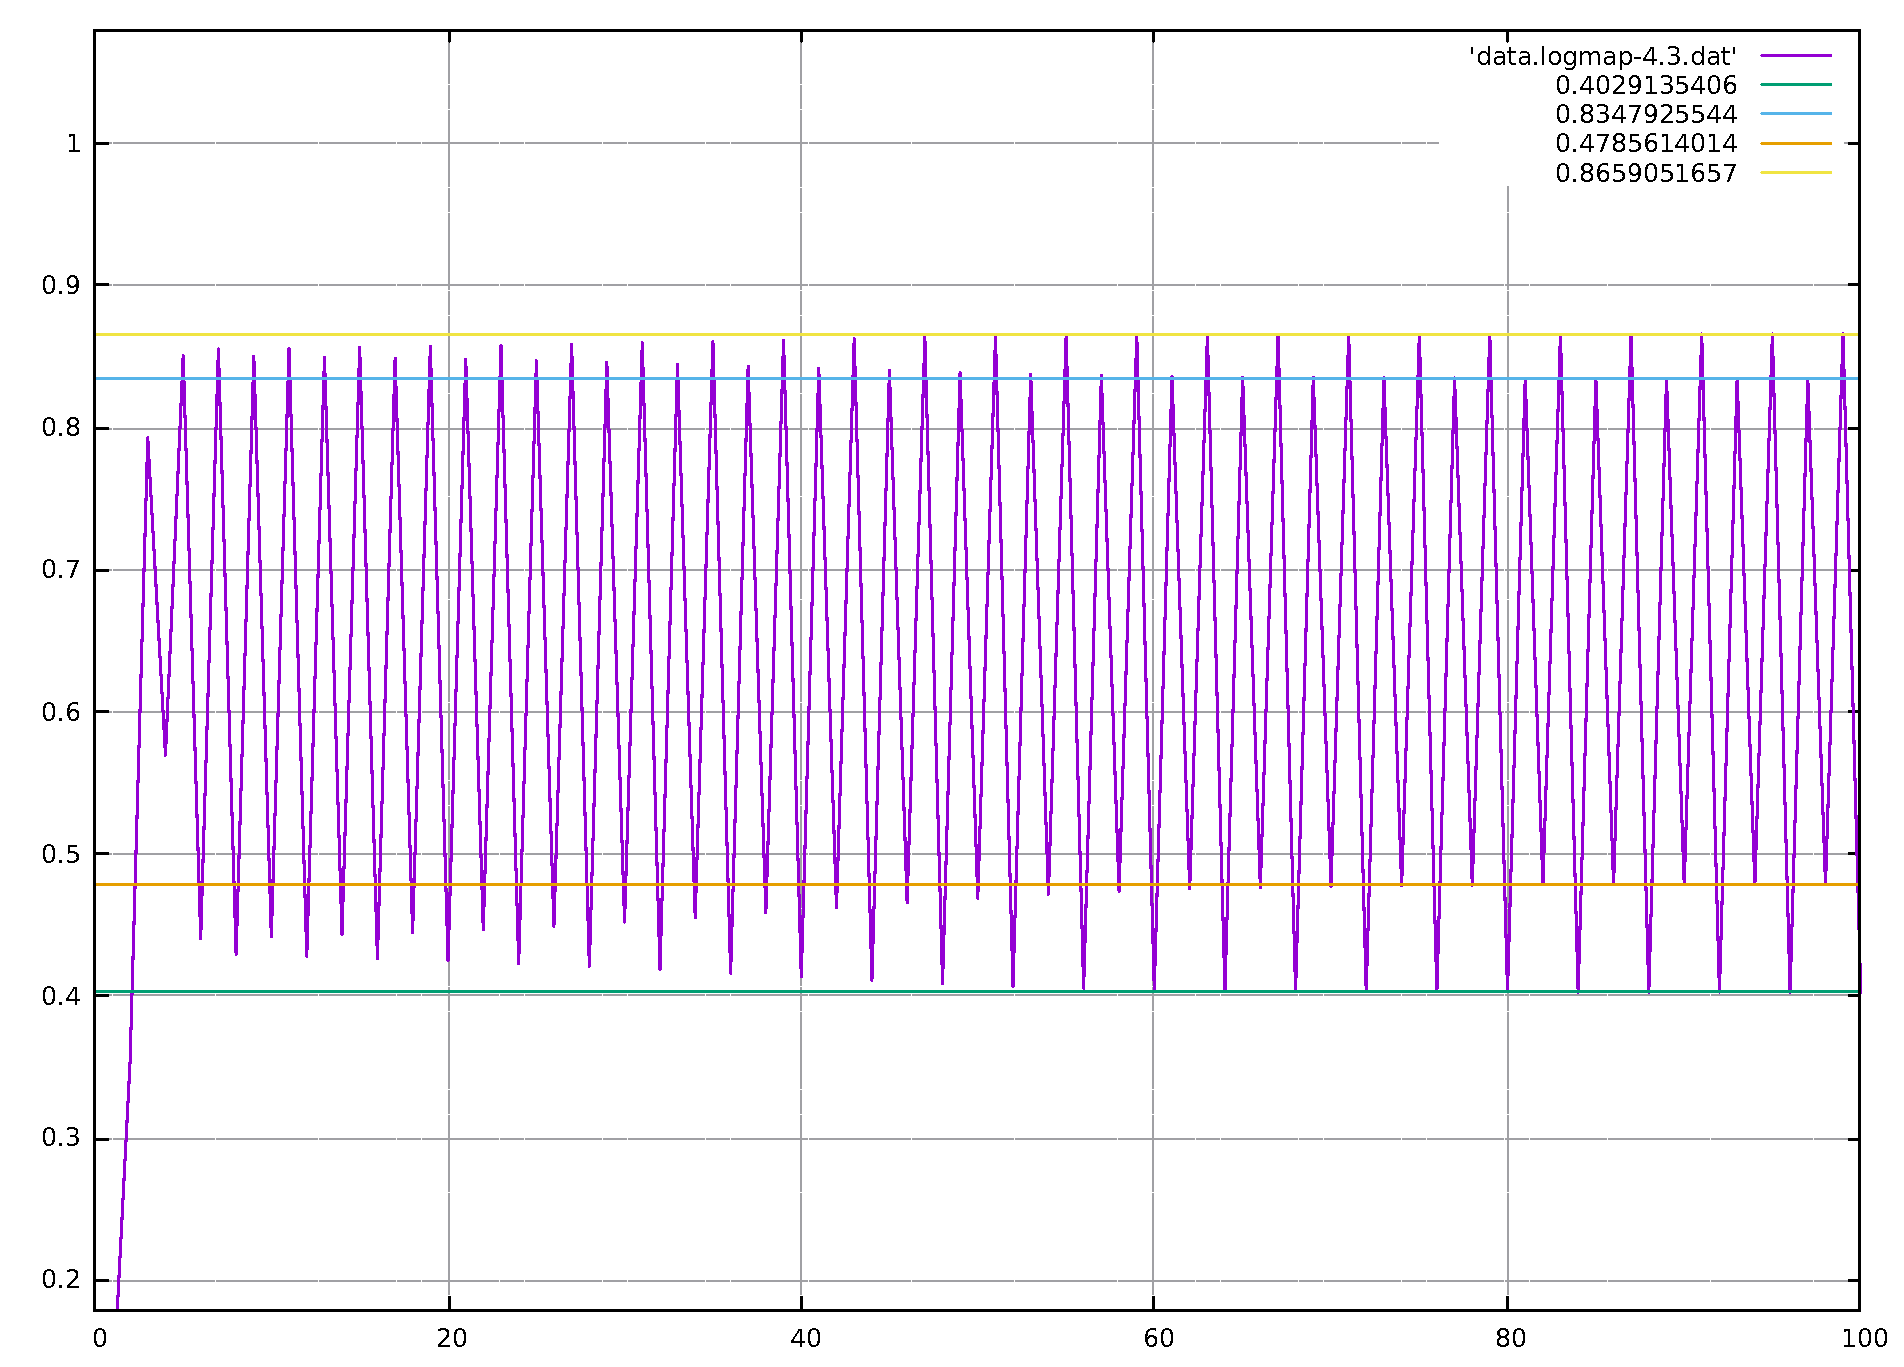
\includegraphics{09}}
\caption*{$x*\ na\ ordenada\ e\ x_{n}\ na\ abscissa$ }
~~~~~~ Vemos neste gráfico que o número de pontos atratores se eleva ao passo que $\lambda$ se eleva.
\end{figure}

\begin{figure}
\subsection{Diagrama para $\lambda = 3.55$}
~~~~~~ Para este caso o diagrama parece ainda mais confuso, possuindo inumeros pontos onde o mapa corta a reta $x' = x$, sendo também maior o distanciamento dos pontos onde o corroe a intersecção.

\centering
\caption{Mapa Escada $\lambda = 3.55$.}
\resizebox{\columnwidth}{!}{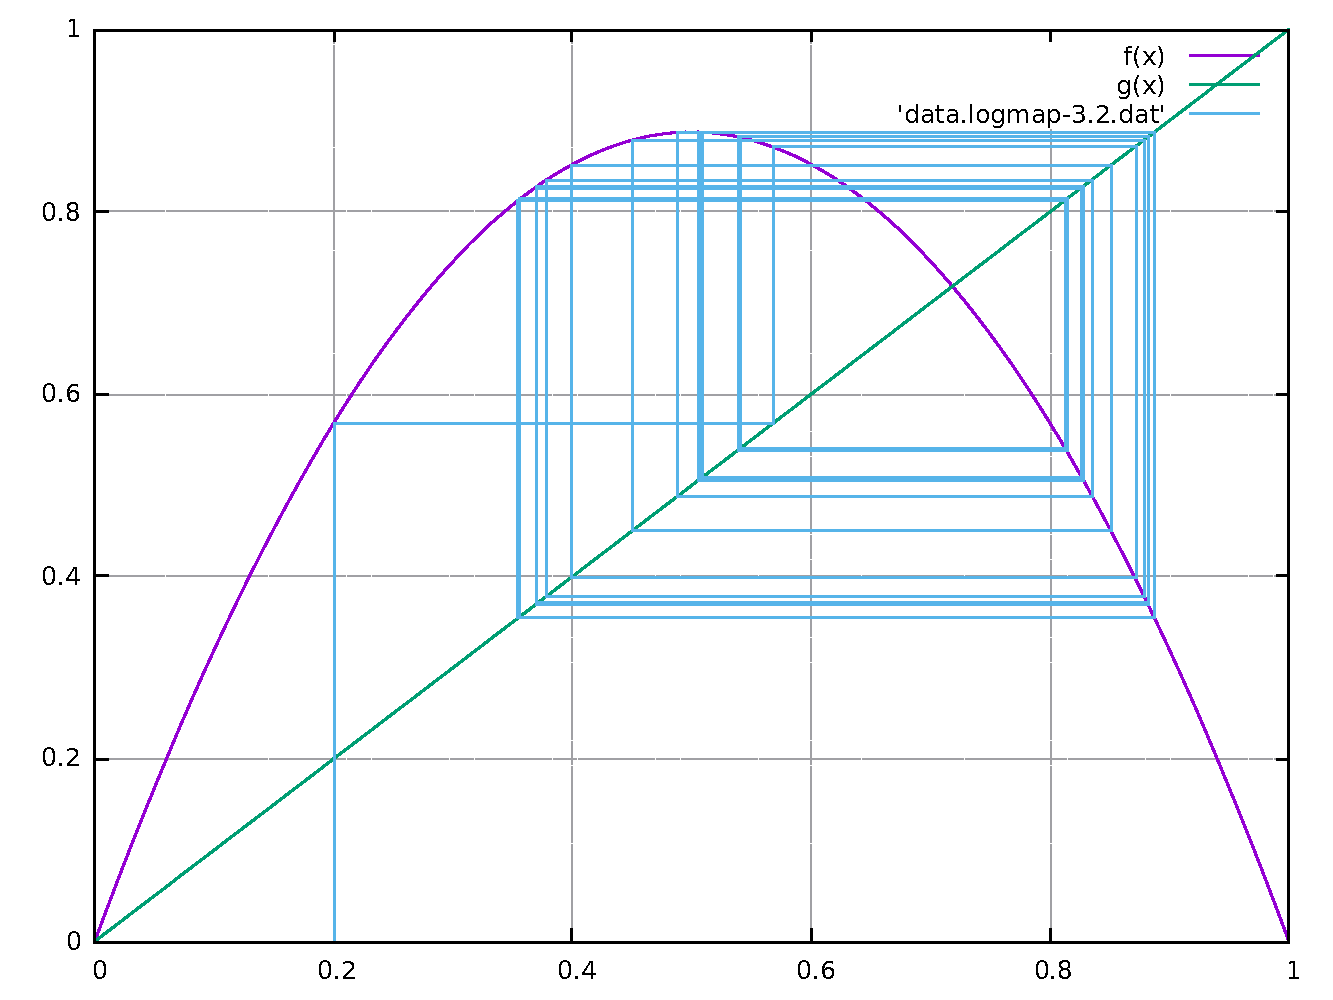
\includegraphics{07}}
\caption*{$x_{n+1}\ na\ ordenada\ e\ x_{n}\ na\ abscissa$ }
\end{figure}

\begin{figure}
~~~~~~ Aqui vemos um aumento exponencial no núnemor de pontos atratores. 
\centering
\caption{Convergência do Mapa Logístico para $\lambda = 3.55$.}
\resizebox{\columnwidth}{!}{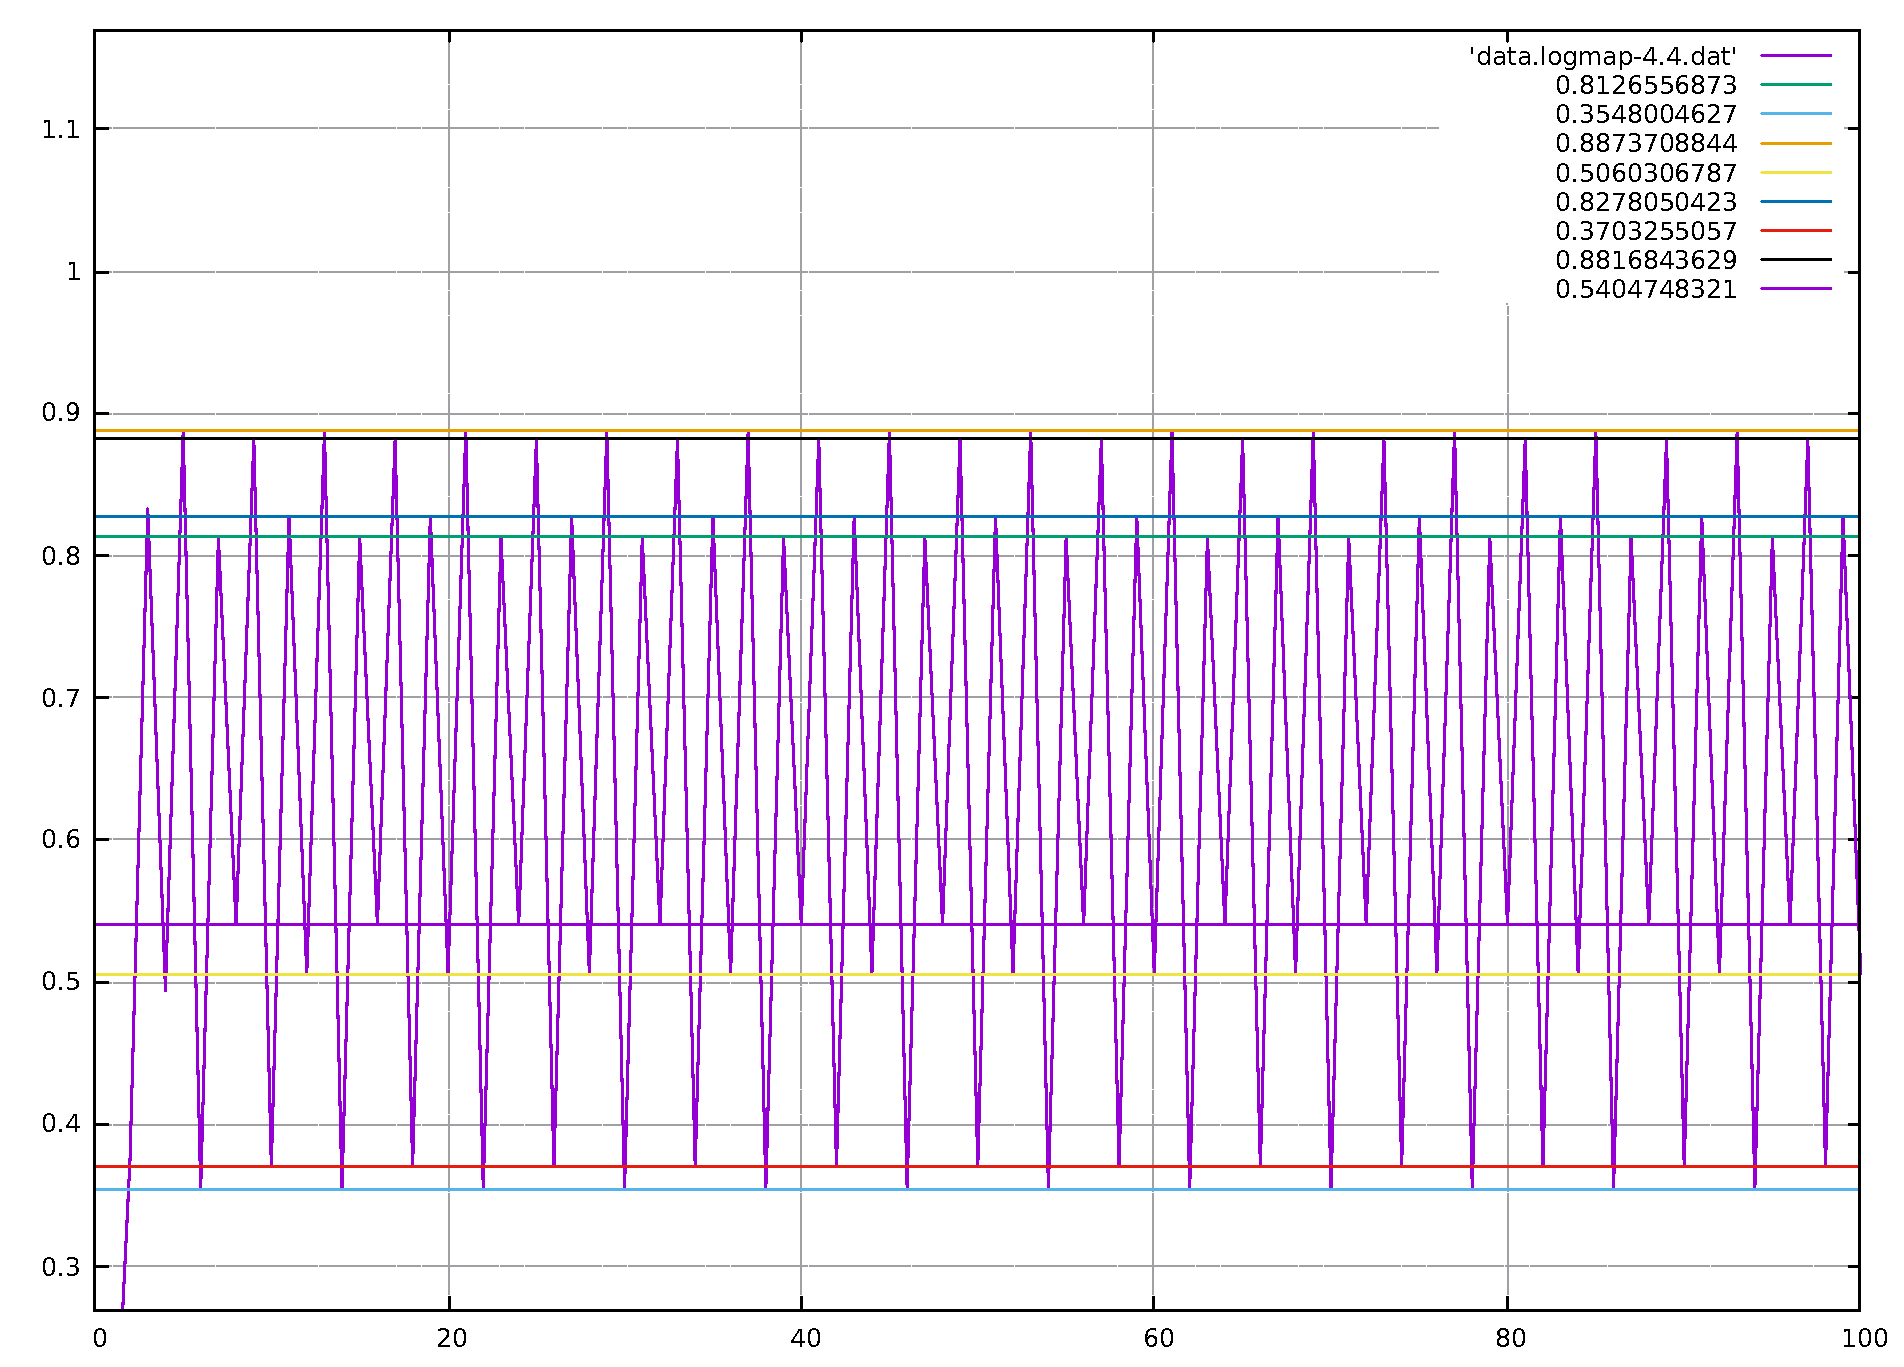
\includegraphics{10}}
\caption*{$x*\ na\ ordenada\ e\ x_{n}\ na\ abscissa$ }\ 

~~~~~~ Este fenômeno ocorre devido a aproximação do valor limite onde seu número tende a uma contagem imensuravel, para $\lambda \leq 4$ podemmos avaliar, sendo melhor visto no mapa bifurcado.
\end{figure}

\begin{figure}
\section{Curvas Próximo ao Ponto Crítico}
~~~~~~ Tornando a avaliar o comportamento temporal para valores de $\lambda$, neste caso se deseja ver o tipo de curva que estas iterações parecem reproduzir, dado que há um decaimento para valores iniciais de $x$ ao realizar as iterações.

\subsection{Caso para $\lambda = 0.90$, inferior ao ponto crítico}
~~~~~~ Aqui temos um caso em que o $\lambda$ está abaixo do ponto crítico.

\centering
\caption{Decaimento temporal, em $\lambda = 0.90$.}
\resizebox{\columnwidth}{!}{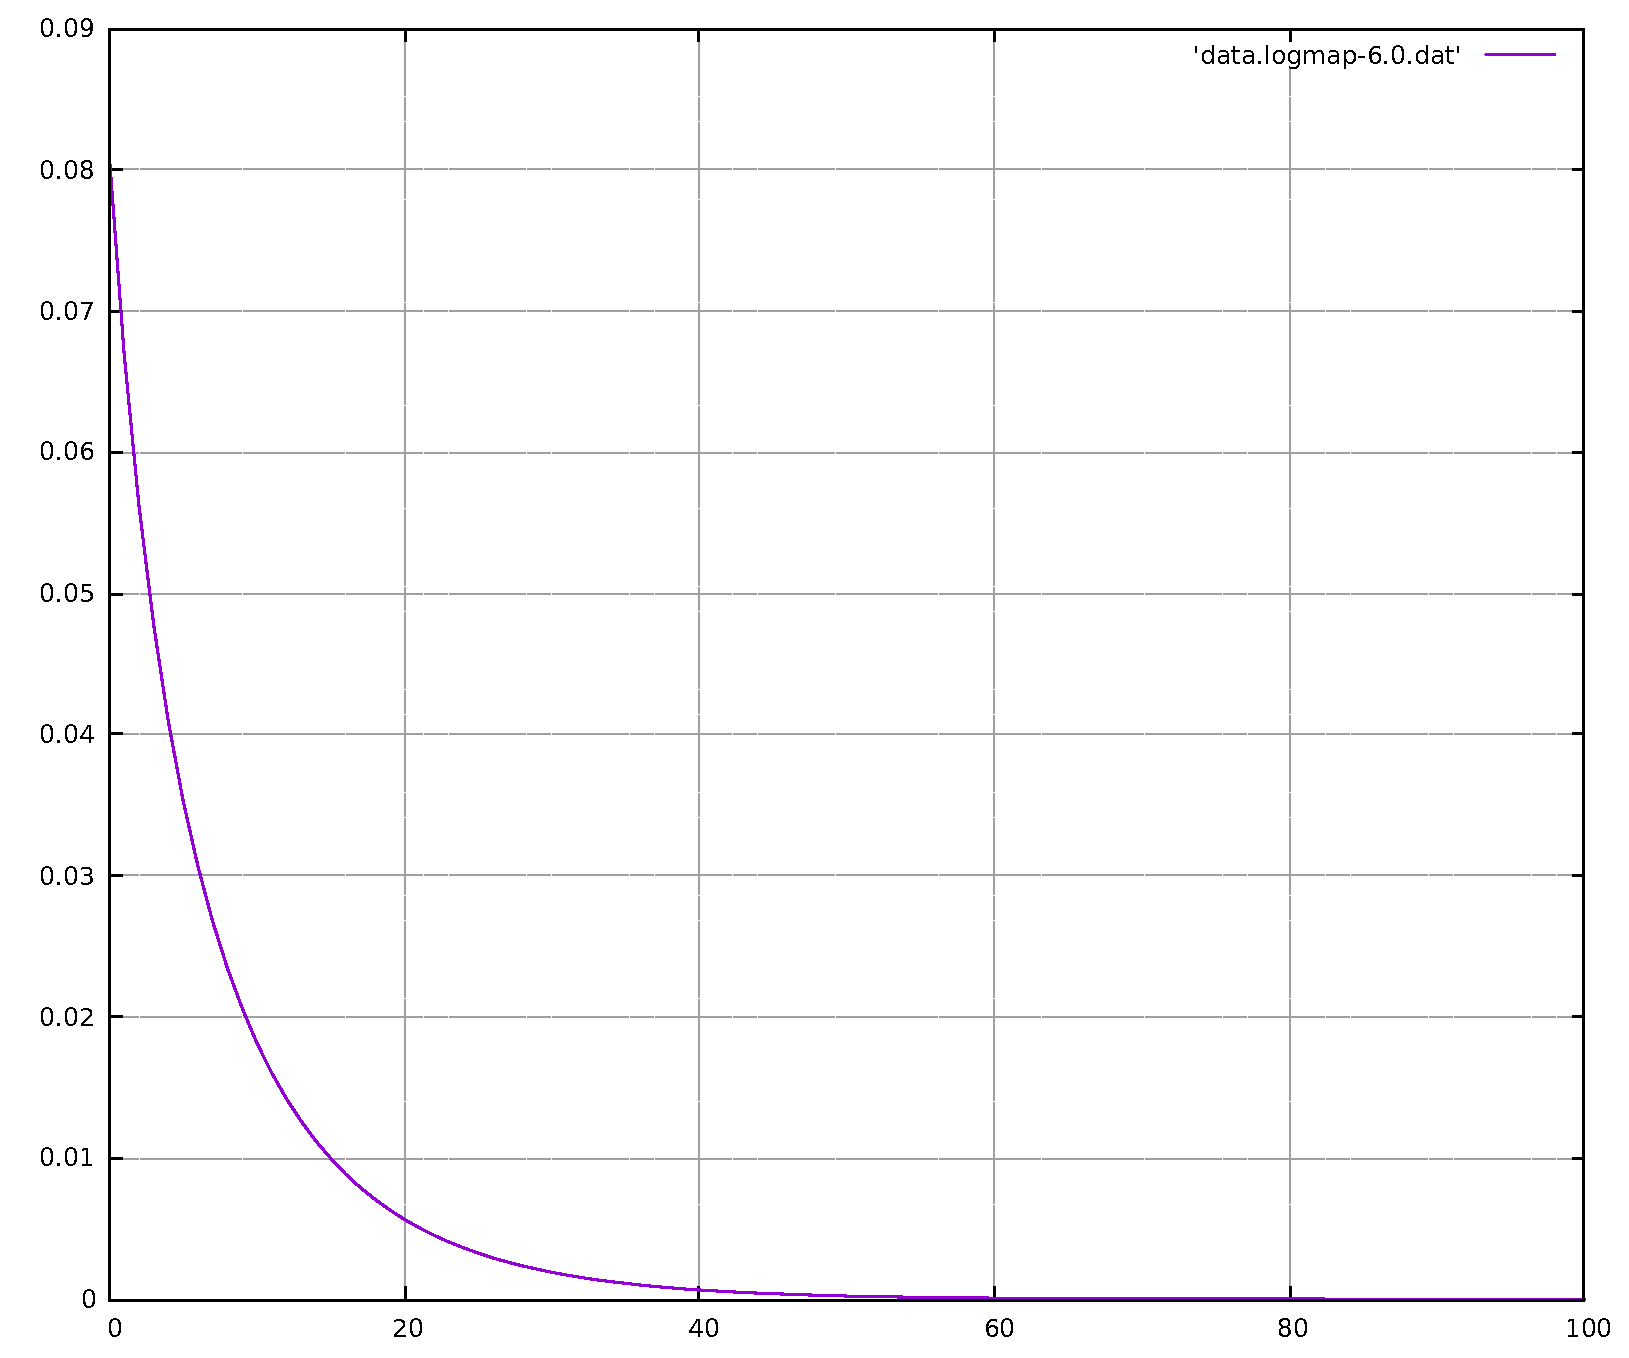
\includegraphics{11}}
\caption*{$x\ na\ ordenada\ e\ tempo(segundos)\ na\ abscissa$}
\end{figure}

\begin{figure}
~~~~~~ Claramente vemos que esta curva não descreve uma lei de potência, sendo apenas um decaimento dado por uma curva genérica.

\centering
\caption{Log $x(t)$ x Log $t$: Verificar lei de potência, em $\lambda = 0.90$.}
\resizebox{\columnwidth}{!}{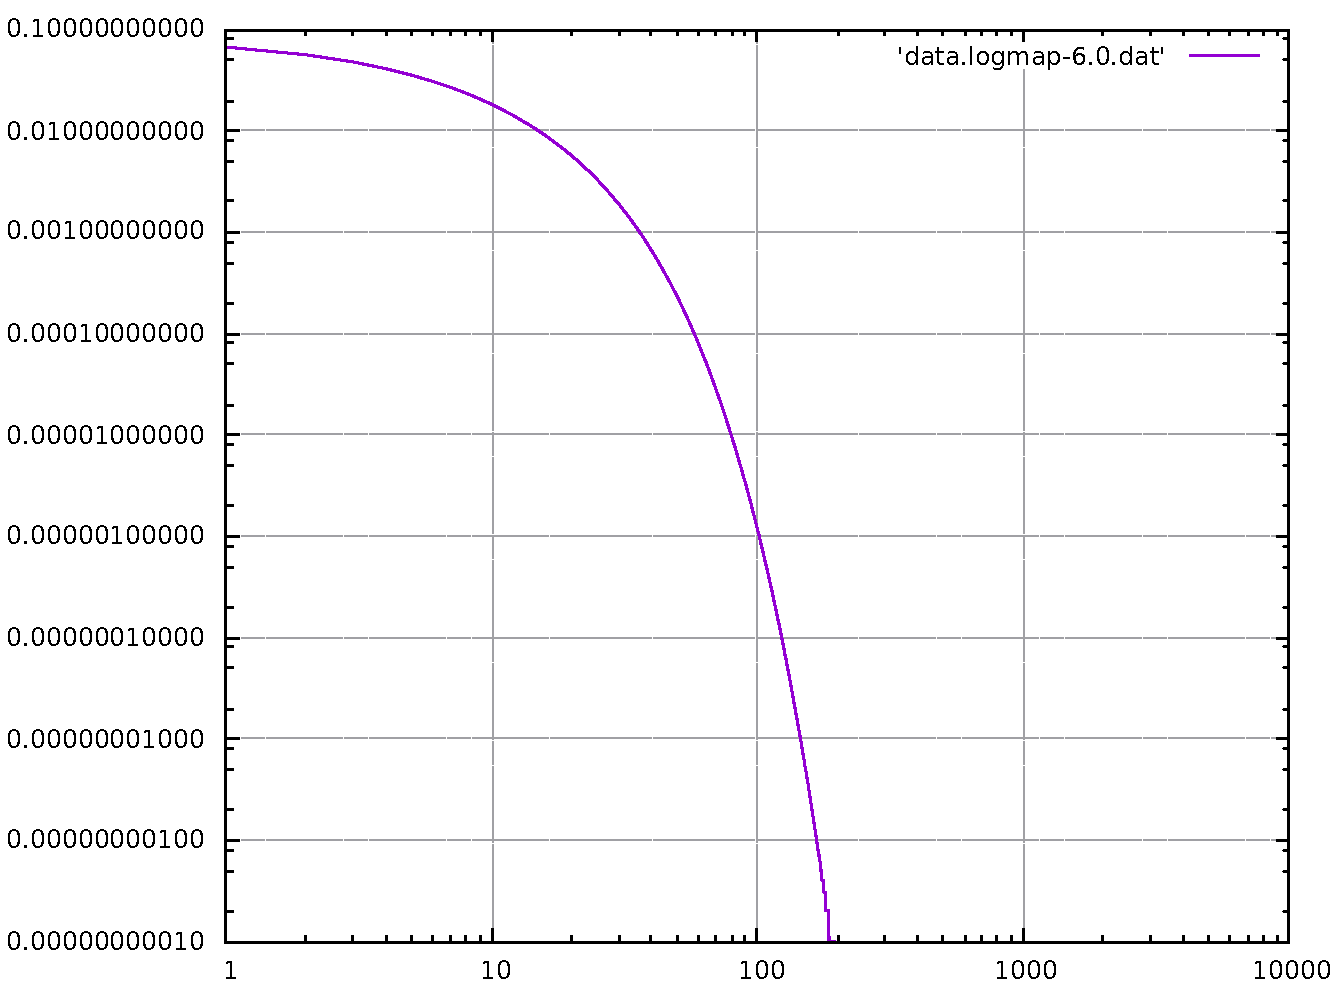
\includegraphics{12}}
\caption*{$x\ na\ ordenada\ e\ tempo(segundos)\ na\ abscissa$}
\end{figure}

\begin{figure}
~~~~~~ Ainda sim podemos realizar um fit por uma função $x(t) = \alpha x^{\beta t}$ via comando GNUplot, obtendo valores $\alpha = 0.101214, \Delta \alpha = 0.003283$ e $\beta = -0.845283, \Delta \beta = 0.02238$ para obter uma curva aproximada.\

\centering
\caption{Ajuste por $x(t) = 0.10t^{-0.85}$, em $\lambda = 0.90$.}
\resizebox{\columnwidth}{!}{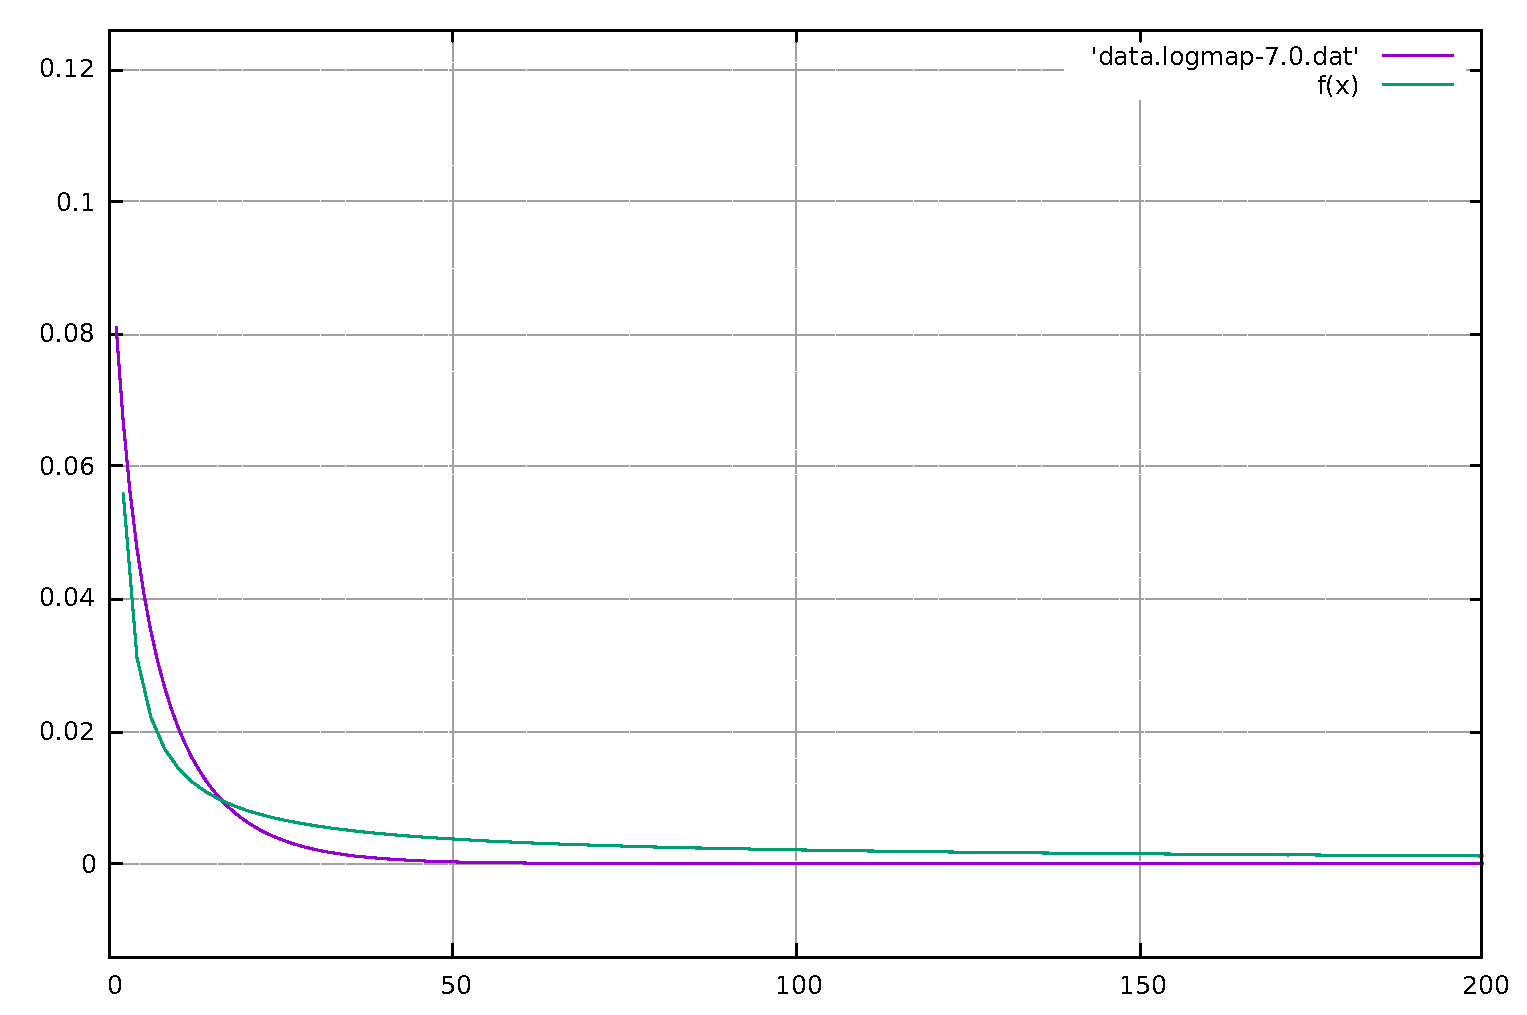
\includegraphics{15}}
\caption*{$x\ na\ ordenada\ e\ tempo(segundos)\ na\ abscissa$}\ 

~~~~~~ Esta curva não representa de fato a lei física a qual o problema descreve, apenas aproxima um conjunto de valores para que tenhamos um parâmetro, sendo um ajuste para uma curva.
\end{figure}

\begin{figure}
\subsection{Caso para $\lambda = 1.00$, no ponto crítico}
~~~~~~ Neste caso se espera ver a mudança de comportamento, dado que $\lambda$ está sobre o ponto crítico.

\centering
\caption{Decaimento temporal, em $\lambda = 1.00$.}
\resizebox{\columnwidth}{!}{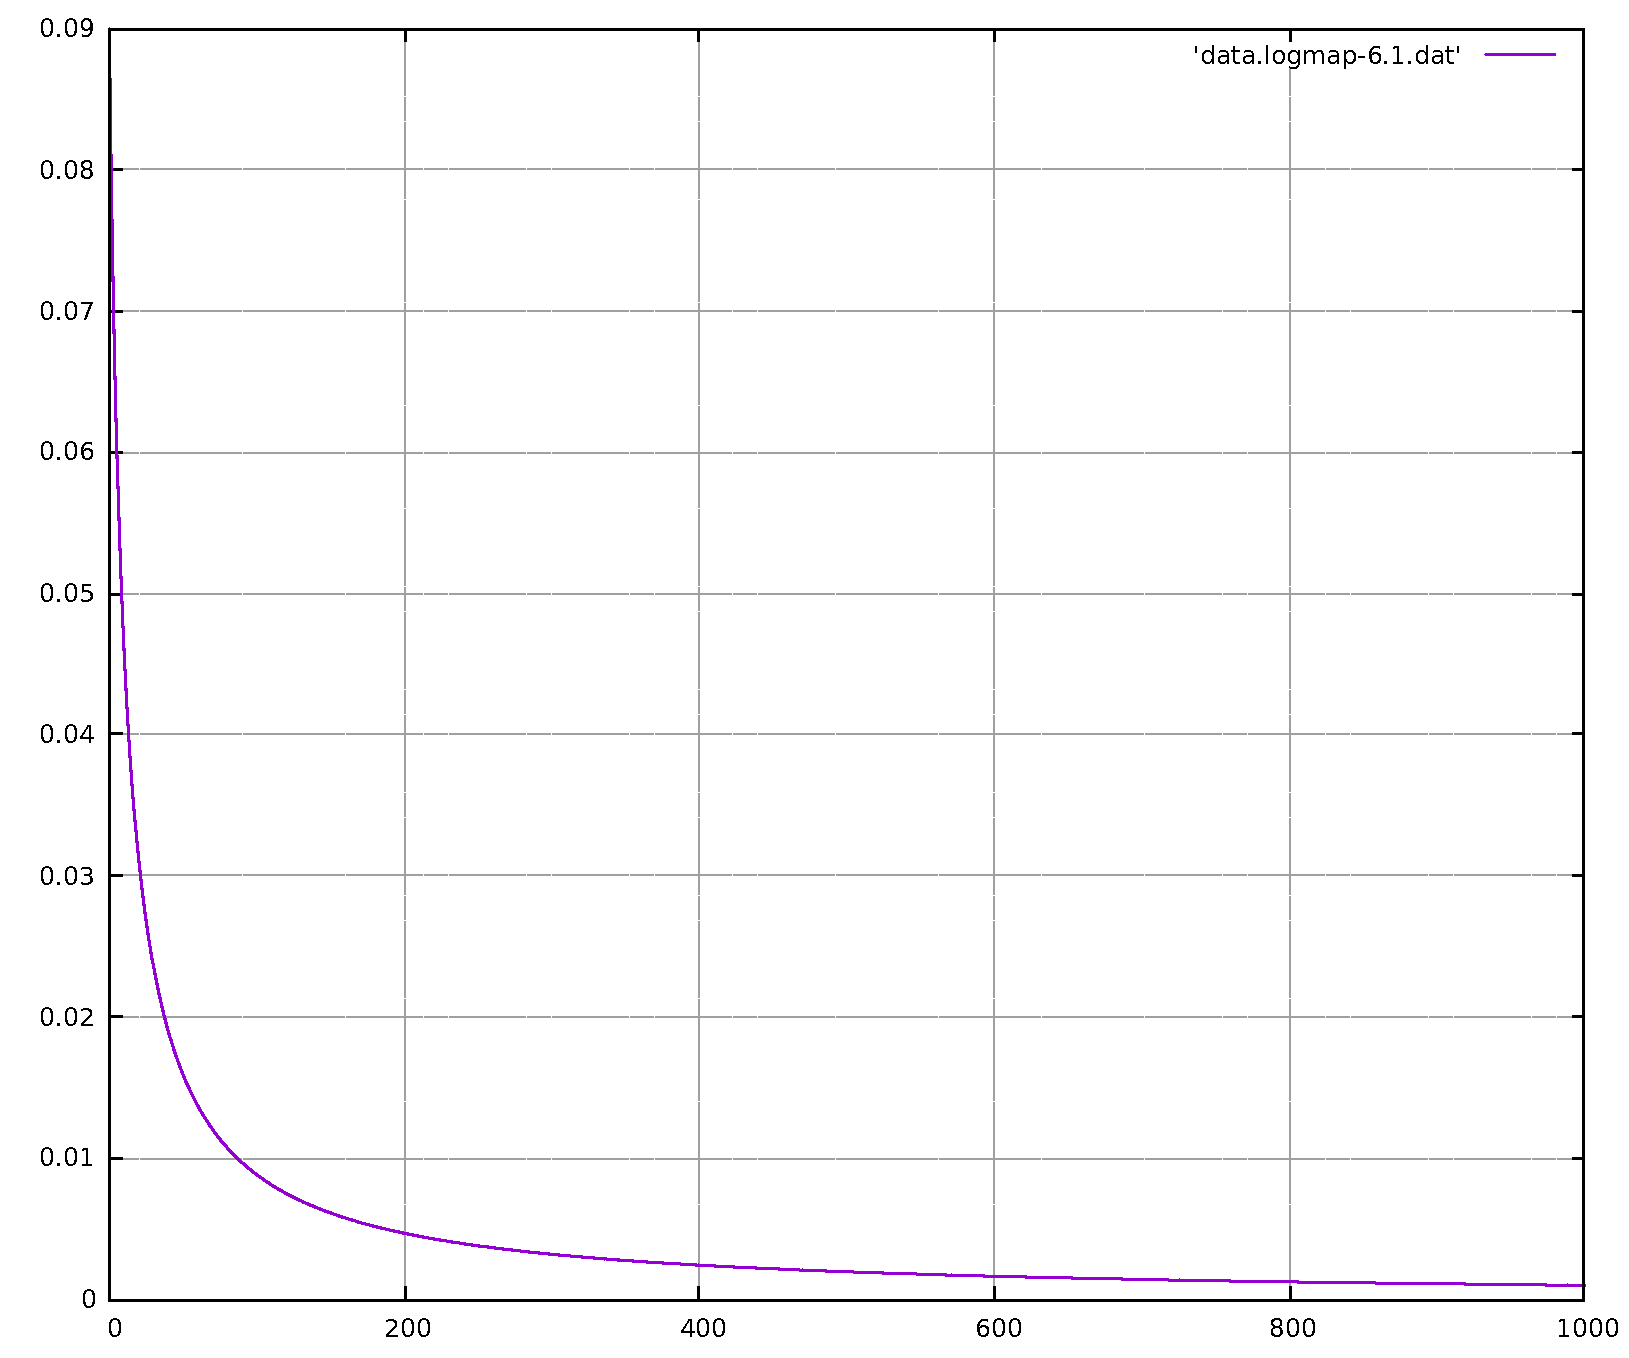
\includegraphics{13}}
\caption*{$x\ na\ ordenada\ e\ tempo(segundos)\ na\ abscissa$}
\end{figure}

\begin{figure}
~~~~~~ Aqui vemos que para valores longos de tempo a curva parece descrever uma lei de potência, ainda que mais próximo a $t\ = 0$ temos um comprtamento estranho, caraterístico de outro tipo de curva que não dada por uma lei de potência.

\centering
\caption{Log $x(t)$ x Log $t$: Verificar lei de potência, em $\lambda = 1.00$.}
\resizebox{\columnwidth}{!}{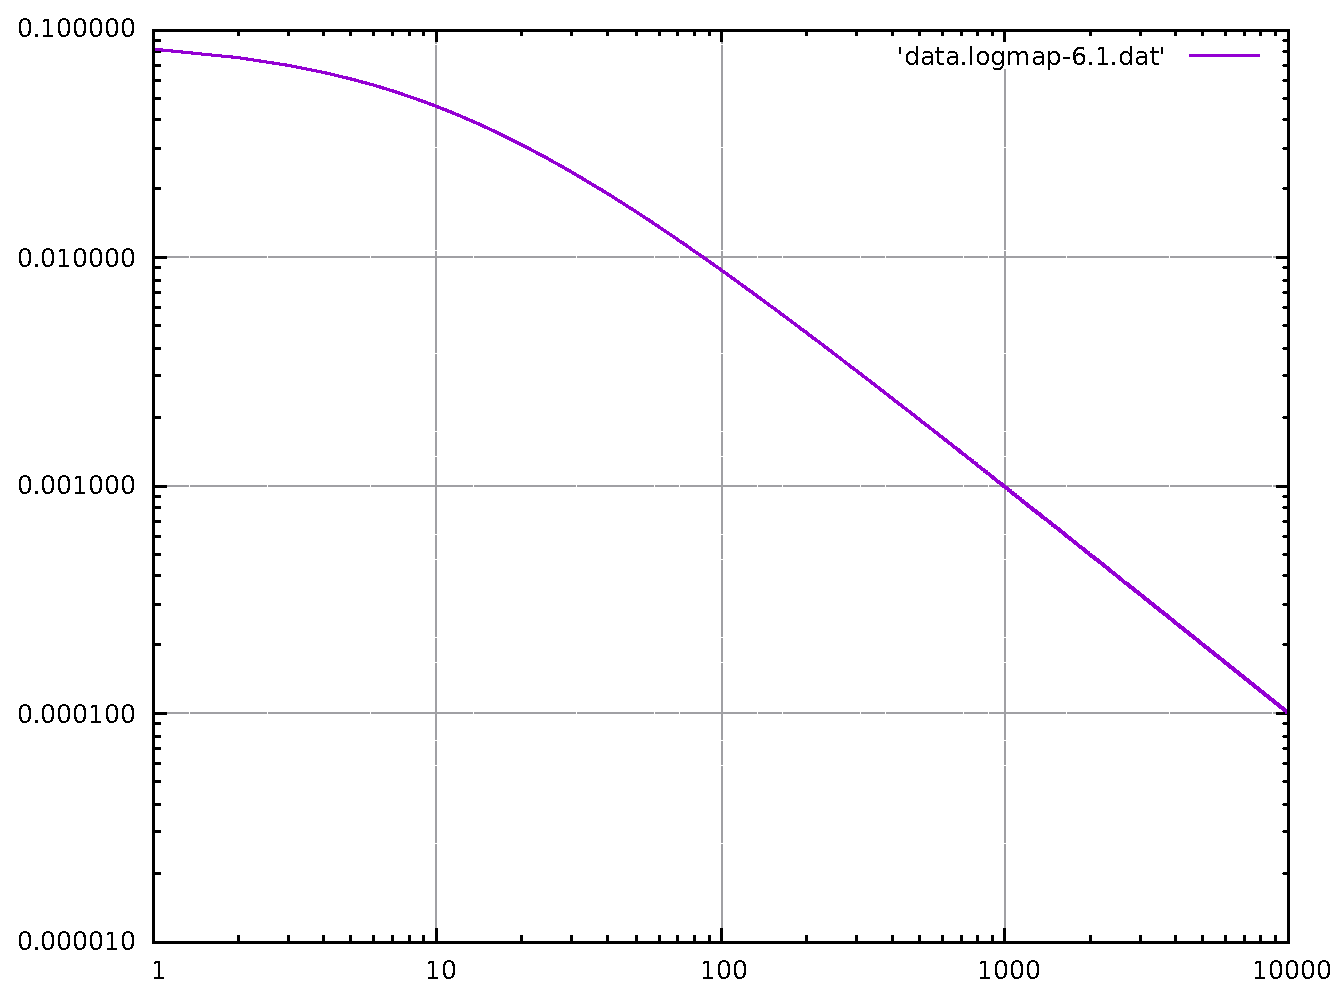
\includegraphics{14}}
\caption*{$x\ na\ ordenada\ e\ tempo(segundos)\ na\ abscissa$}
\end{figure}

\begin{figure}

~~~~~~ Tornando ao fit, podemos usar para este conjunto de pontos o mesmo recurso via GNUplot, obtendo $\alpha = 0.121861, \Delta \alpha = 0.003245$ e $\beta = -0.515002, \Delta \beta = 0.0094$.

\centering
\caption{Ajuste por $x(t) = 0.12t^{-0.52}$, em $\lambda = 1.00$.}
\resizebox{\columnwidth}{!}{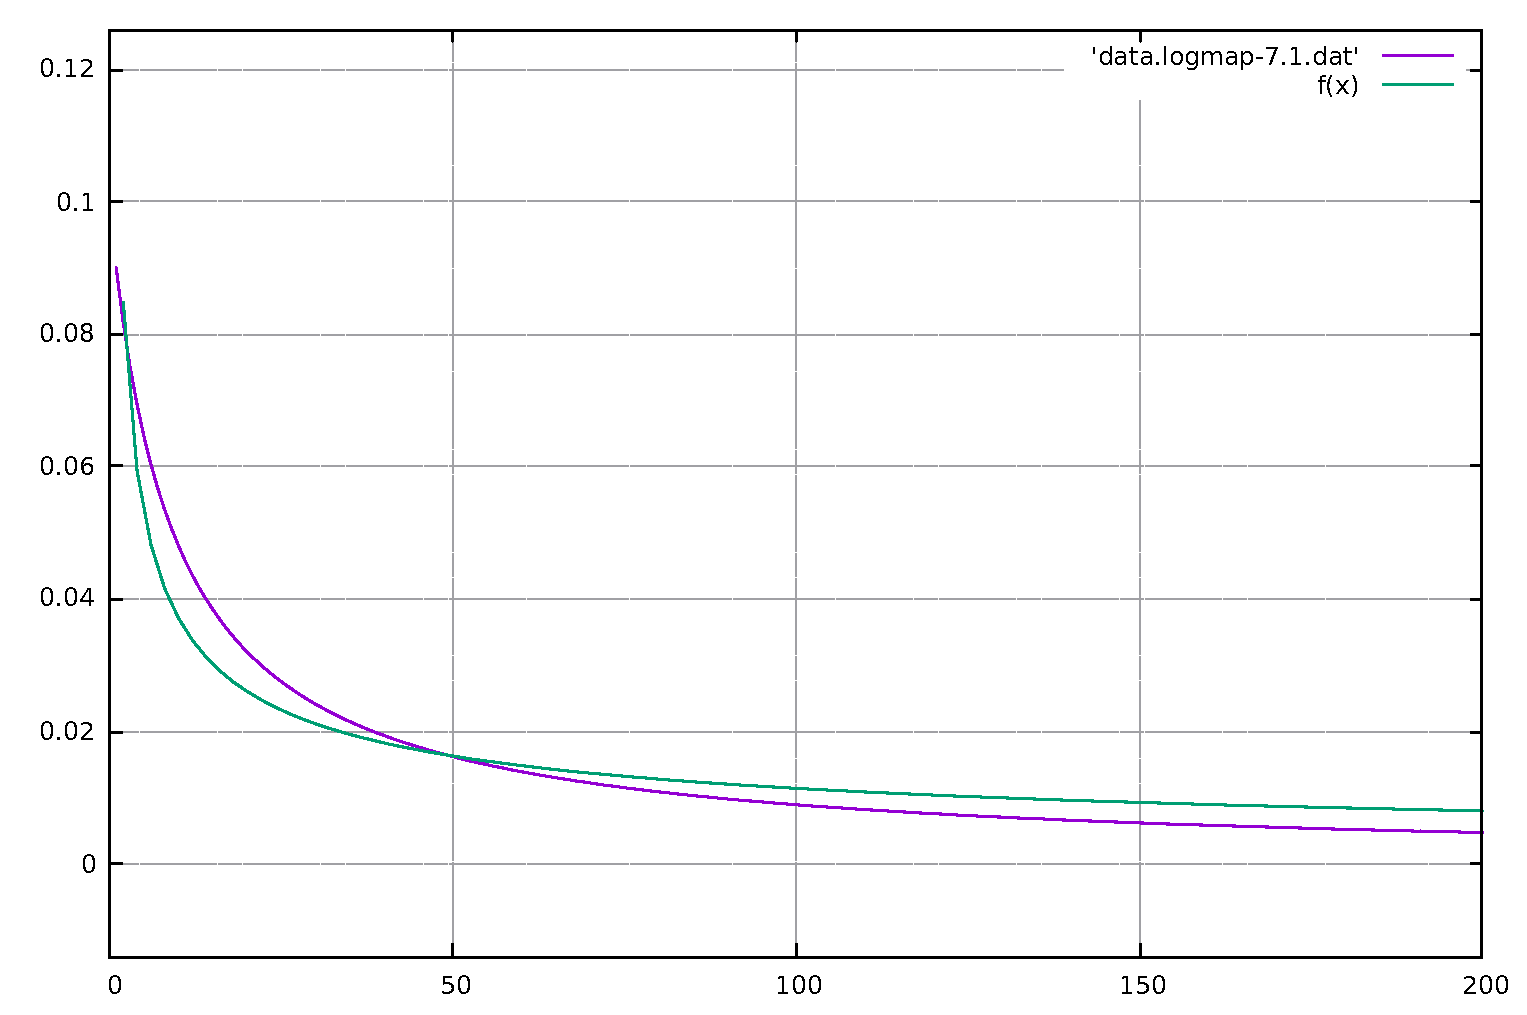
\includegraphics{16}}
\caption*{$x\ na\ ordenada\ e\ tempo(segundos)\ na\ abscissa$}
\end{figure}
\begin{figure}

\section{Mapa Bifurcado}

\subsection{Atratores Estranhos}

~~~~~~ Para consumar este trabalho, temos um plote dos pontos de $\lambda$. O longo deste texto fiz mensão diversas vezes a transição e os pontos de $\lambda$. Aqui vemos a relação direta entre os possíveis valores de $x*$ em função da disribuição de $\lambda$, onde contemplamos este mapa conhecido como: Mapa Bifurcado.  Sendo em $\lambda = 4$ um grande númerio de pontos atratores, aparentemente crescente de forma caótica e indeterminada. Tal efeito é oriundo de observarmos muito proximo a evolução temporal do nosso sistema, para tempos maiores devemos notar algum padrão mais geral.

\centering
\caption{$0 \leq \lambda \leq 4.00$.}
\resizebox{\columnwidth}{!}{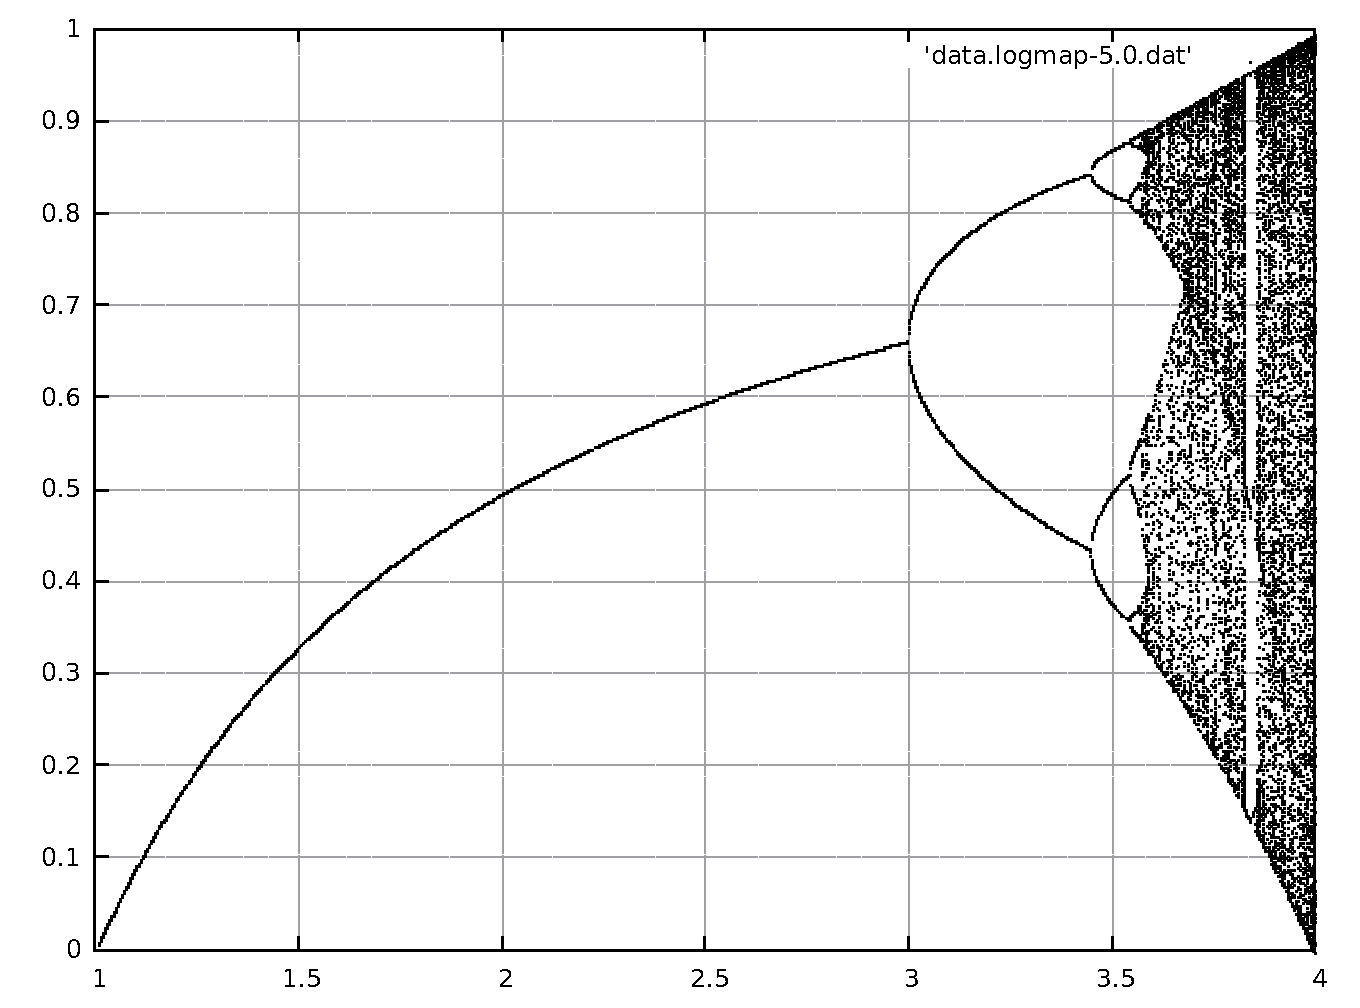
\includegraphics{forkmap}}
\caption*{ $x*\ na\ ordenada\ e\ \lambda\ na\ abscissa$ }
\end{figure}

\end{document}